\documentclass[11pt, a4paper, twoside]{article}   	% use "amsart" instead of "article" for AMSLaTeX format

\usepackage{geometry}                		% See geometry.pdf to learn the layout options. There are lots.
\usepackage{pdfpages}
\usepackage{caption}
\usepackage{minted}
\usepackage[german]{babel}			% this end the next are needed for german umlaute
\usepackage[utf8]{inputenc}
\usepackage{color}
\usepackage{graphicx}
\usepackage{titlesec}
\usepackage{fancyhdr}
\usepackage{lastpage}
\usepackage{hyperref}
\usepackage[autostyle=false, style=english]{csquotes}
\usepackage{mathtools}
\usepackage{tabularx}
% http://www.artofproblemsolving.com/wiki/index.php/LaTeX:Symbols#Operators
% =============================================
% Layout & Colors
% =============================================
\geometry{
   a4paper,
   total={210mm,297mm},
   left=20mm,
   right=20mm,
   top=20mm,
   bottom=30mm
 }	

\definecolor{myred}{rgb}{0.8,0,0}
\definecolor{mygreen}{rgb}{0,0.6,0}
\definecolor{mygray}{rgb}{0.5,0.5,0.5}
\definecolor{mymauve}{rgb}{0.58,0,0.82}

\setcounter{secnumdepth}{4}


% the default java directory structure and the main packages
\newcommand{\srcDir}{../src/ImageJ/plugins/bva2}
\newcommand{\imageDir}{images}


% =============================================
% Code Settings
% =============================================
\newenvironment{code}{\captionsetup{type=listing}}{}
\newmintedfile[javaFile]{java}{
	linenos=true, 
	frame=single, 
	breaklines=true, 
	tabsize=2,
	numbersep=5pt,
	xleftmargin=10pt,
	baselinestretch=1,
	fontsize=\footnotesize
}

\newmintinline[inlineJava]{java}{}
\newminted[javaSource]{java}{
	breaklines=true, 
	tabsize=2,
	autogobble=true,
	breakautoindent=false
}


\newcommand{\xvdash}[1]{%
  \vdash^{\mkern-10mu\scriptscriptstyle\rule[-.9ex]{0pt}{0pt}#1}%
}

% =============================================
% Page Style, Footers & Headers, Title
% =============================================
\title{Übung 6}
\author{Gattringer Marko, Ruhsam Christoph}

\lhead{Gattringer Marko, Ruhsam Christoph}
\chead{BVA}
\rhead{Übung 6}

\lfoot{S1810454012, S1810454036}
\cfoot{}
\rfoot{ \thepage / \pageref{LastPage} }
\renewcommand{\footrulewidth}{0.4pt}
% =============================================
% D O C U M E N T     C O N T E N T
% =============================================
% =============================================
% 2016.10.13: 1 
% 2016.10.14: 2
% =============================================
\pagestyle{fancy}
\begin{document}
\setlength{\headheight}{15mm}
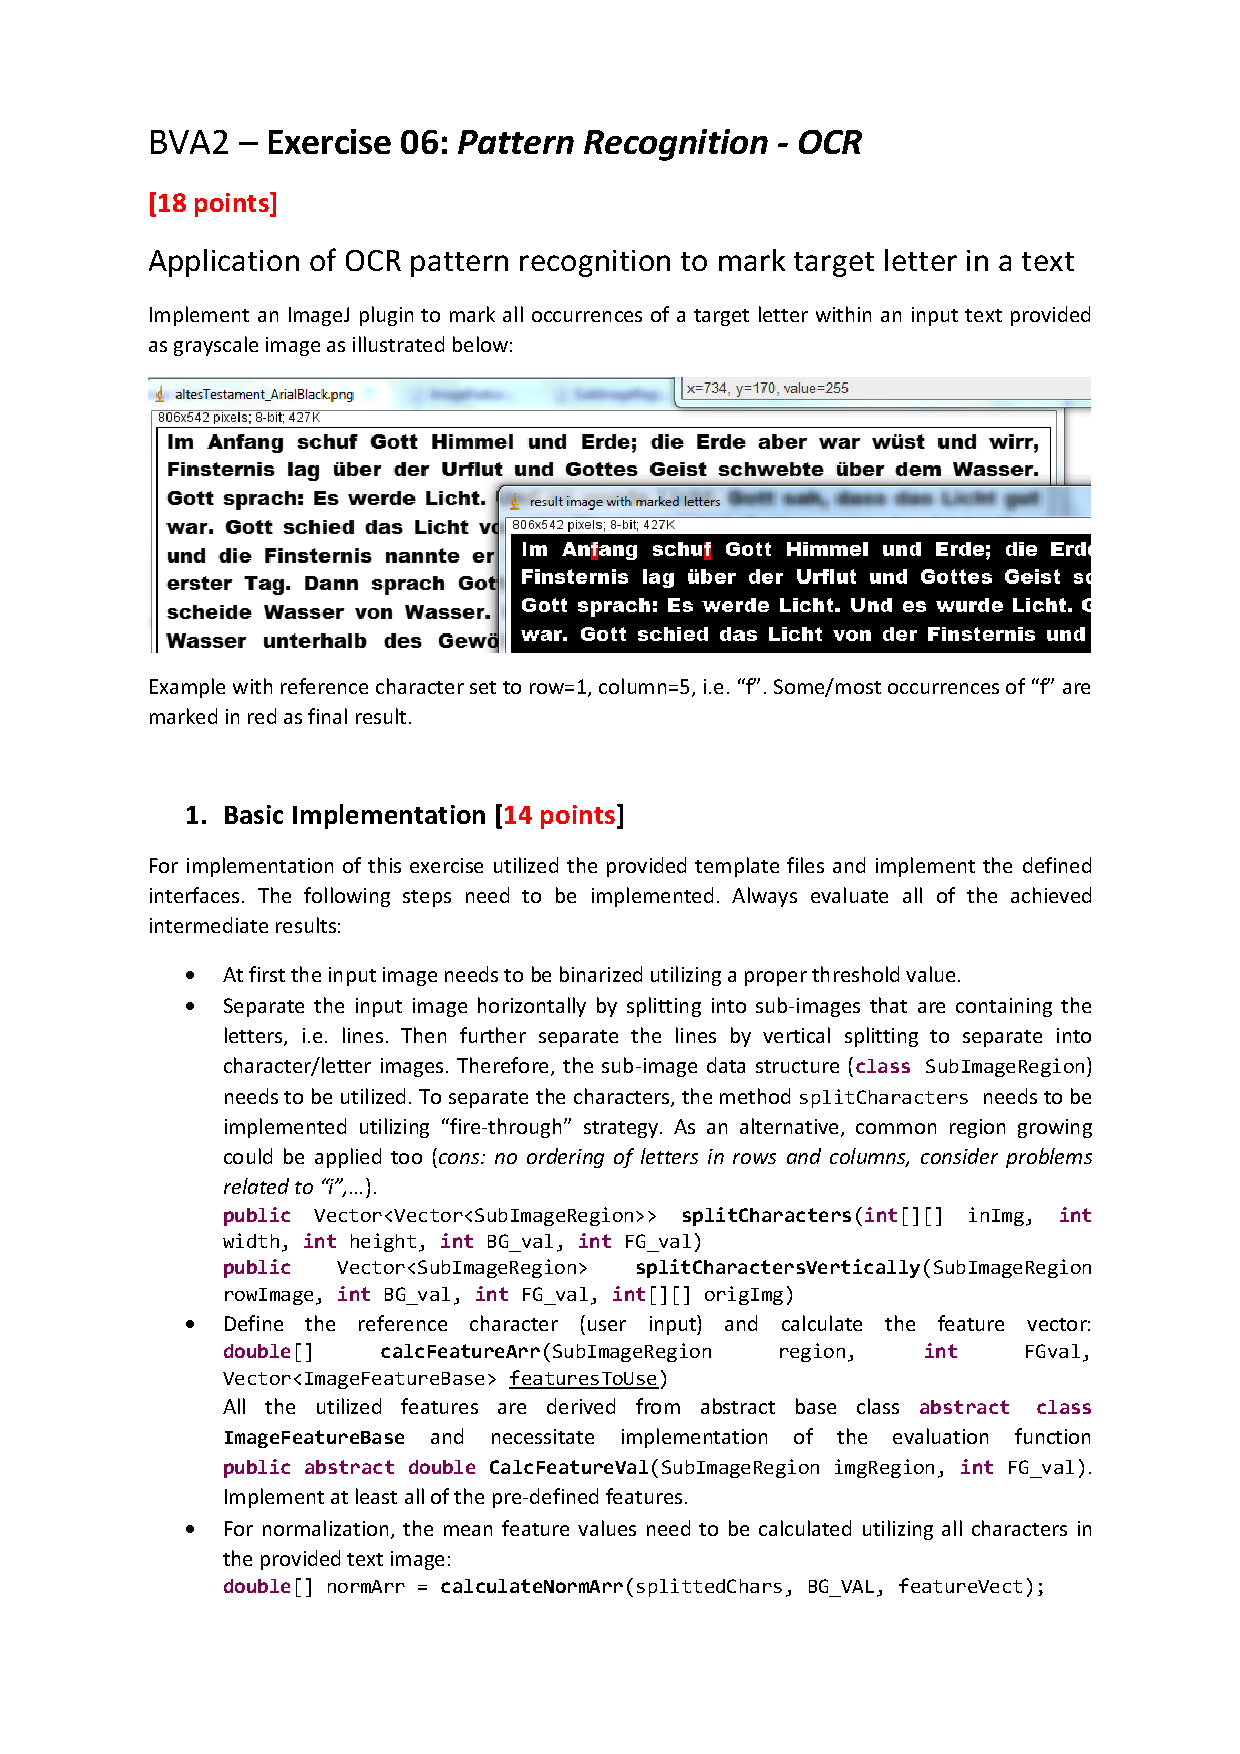
\includepdf[pages={1,2}]{Angabe.pdf}


\section{Basic Implementation}
\subsection{Lösungsidee}
%TODO
TODO

\subsubsection{Features}

\begin{itemize}
	\item \textbf{F1: number of pixels: } %TODO Christoph
	\item \textbf{F2: extent in x-direction (max width): }  %TODO Christoph
	\item \textbf{F3: extent in y-direction (max height): } %TODO Christoph
	
	\item \textbf{F4: average distance from centroid: } Zuerst wird die Berechnung des Zentroide in einer eigenen Hilfsfunktion implementiert, welche später auch für die restlichen Features (die den Zentroiden benötigen) verwendet werden kann. Die X-Koordinate des Zentroiden wird bestimmt, indem alle X-Koordinaten der Pixel, die zum jeweiligen Buchstaben gehören, aufsummiert werden und durch die Anzahl der beteiligten Pixel dividiert werden. Für die Y-Koordinate werden dann die jeweiligen y-Koordinaten aufsummiert. 
	Um die durchschnittliche Distanz zum Zentroiden zu berechnen werden alle Distanzen zu allen Pixeln die zum Buchstaben gehören aufsummiert und durch die Anzahl der Pixel geteilit. Zum bestimmen der Distanz wird die Formel $\sqrt{((x\textsubscript{2} - x\textsubscript{1})^2 + (y\textsubscript{2} - y\textsubscript{1})^2)}$ verwendet.
	
	\item \textbf{F5: min distance from centroid: } Um die minimale Distanz zum Zentroiden zu bestimmen wird der Zentroide wieder mit der zuvor implementierten Hilfsfunktion bestimmt, um dann die minimale Distanz zu finden.
	
	\item \textbf{F6: max distance from centroid: } Funktioniert gleich wie das Bestimmen der minimalen Distanz, nur das hier die maximale Distanz als Ergebnis gespeichert wird.
	
	\item \textbf{F7: circularity: } Zur Berechnung der \enquote{Circularity} wirde folgende Formel herangezogen:\\ $circularity = \frac{4\pi * area}{perimeter^2}$. Wobei \enquote{area} die Anzahl der Pixel eines Zeichens und \enquote{perimeter} die Anzahl der Pixel des Umfangs sind. Beide Werte können über die ImageJ-Klasse \enquote{Analyzer} ermittelt werden.
	
	\item \textbf{F8: rel pos centroid within bounding box, x-direction: } Zur Berechnung des Zentroiden kann wieder die Hilfsfunktion von vorher verwendet werden. Danach kann die relative Position in x-Richtung berechnet werden.
	
	\item \textbf{F9: rel pos centroid within bounding box, y-direction: } Funktioniert Äquivalent zu F8, nur das hier die Position in y-Richtung berechnet wird.
	
\end{itemize}

\subsection{Ausarbeitung}
\begin{code}
	\caption{OCRanalysis\_.java}
	\javaFile{\srcDir/OCRanalysis_.java}
	\label{src:exercise-OCRanalysis-java}
\end{code}

\subsection{Tests}

\end{document}